
% Default to the notebook output style

    


% Inherit from the specified cell style.




    
\documentclass[11pt]{article}

    
    
    \usepackage[T1]{fontenc}
    % Nicer default font (+ math font) than Computer Modern for most use cases
    \usepackage{mathpazo}

    % Basic figure setup, for now with no caption control since it's done
    % automatically by Pandoc (which extracts ![](path) syntax from Markdown).
    \usepackage{graphicx}
    % We will generate all images so they have a width \maxwidth. This means
    % that they will get their normal width if they fit onto the page, but
    % are scaled down if they would overflow the margins.
    \makeatletter
    \def\maxwidth{\ifdim\Gin@nat@width>\linewidth\linewidth
    \else\Gin@nat@width\fi}
    \makeatother
    \let\Oldincludegraphics\includegraphics
    % Set max figure width to be 80% of text width, for now hardcoded.
    \renewcommand{\includegraphics}[1]{\Oldincludegraphics[width=.8\maxwidth]{#1}}
    % Ensure that by default, figures have no caption (until we provide a
    % proper Figure object with a Caption API and a way to capture that
    % in the conversion process - todo).
    \usepackage{caption}
    \DeclareCaptionLabelFormat{nolabel}{}
    \captionsetup{labelformat=nolabel}

    \usepackage{adjustbox} % Used to constrain images to a maximum size 
    \usepackage{xcolor} % Allow colors to be defined
    \usepackage{enumerate} % Needed for markdown enumerations to work
    \usepackage{geometry} % Used to adjust the document margins
    \usepackage{amsmath} % Equations
    \usepackage{amssymb} % Equations
    \usepackage{textcomp} % defines textquotesingle
    % Hack from http://tex.stackexchange.com/a/47451/13684:
    \AtBeginDocument{%
        \def\PYZsq{\textquotesingle}% Upright quotes in Pygmentized code
    }
    \usepackage{upquote} % Upright quotes for verbatim code
    \usepackage{eurosym} % defines \euro
    \usepackage[mathletters]{ucs} % Extended unicode (utf-8) support
    \usepackage[utf8x]{inputenc} % Allow utf-8 characters in the tex document
    \usepackage{fancyvrb} % verbatim replacement that allows latex
    \usepackage{grffile} % extends the file name processing of package graphics 
                         % to support a larger range 
    % The hyperref package gives us a pdf with properly built
    % internal navigation ('pdf bookmarks' for the table of contents,
    % internal cross-reference links, web links for URLs, etc.)
    \usepackage{hyperref}
    \usepackage{longtable} % longtable support required by pandoc >1.10
    \usepackage{booktabs}  % table support for pandoc > 1.12.2
    \usepackage[inline]{enumitem} % IRkernel/repr support (it uses the enumerate* environment)
    \usepackage[normalem]{ulem} % ulem is needed to support strikethroughs (\sout)
                                % normalem makes italics be italics, not underlines
    \usepackage{mathrsfs}
    

    
    
    % Colors for the hyperref package
    \definecolor{urlcolor}{rgb}{0,.145,.698}
    \definecolor{linkcolor}{rgb}{.71,0.21,0.01}
    \definecolor{citecolor}{rgb}{.12,.54,.11}

    % ANSI colors
    \definecolor{ansi-black}{HTML}{3E424D}
    \definecolor{ansi-black-intense}{HTML}{282C36}
    \definecolor{ansi-red}{HTML}{E75C58}
    \definecolor{ansi-red-intense}{HTML}{B22B31}
    \definecolor{ansi-green}{HTML}{00A250}
    \definecolor{ansi-green-intense}{HTML}{007427}
    \definecolor{ansi-yellow}{HTML}{DDB62B}
    \definecolor{ansi-yellow-intense}{HTML}{B27D12}
    \definecolor{ansi-blue}{HTML}{208FFB}
    \definecolor{ansi-blue-intense}{HTML}{0065CA}
    \definecolor{ansi-magenta}{HTML}{D160C4}
    \definecolor{ansi-magenta-intense}{HTML}{A03196}
    \definecolor{ansi-cyan}{HTML}{60C6C8}
    \definecolor{ansi-cyan-intense}{HTML}{258F8F}
    \definecolor{ansi-white}{HTML}{C5C1B4}
    \definecolor{ansi-white-intense}{HTML}{A1A6B2}
    \definecolor{ansi-default-inverse-fg}{HTML}{FFFFFF}
    \definecolor{ansi-default-inverse-bg}{HTML}{000000}

    % commands and environments needed by pandoc snippets
    % extracted from the output of `pandoc -s`
    \providecommand{\tightlist}{%
      \setlength{\itemsep}{0pt}\setlength{\parskip}{0pt}}
    \DefineVerbatimEnvironment{Highlighting}{Verbatim}{commandchars=\\\{\}}
    % Add ',fontsize=\small' for more characters per line
    \newenvironment{Shaded}{}{}
    \newcommand{\KeywordTok}[1]{\textcolor[rgb]{0.00,0.44,0.13}{\textbf{{#1}}}}
    \newcommand{\DataTypeTok}[1]{\textcolor[rgb]{0.56,0.13,0.00}{{#1}}}
    \newcommand{\DecValTok}[1]{\textcolor[rgb]{0.25,0.63,0.44}{{#1}}}
    \newcommand{\BaseNTok}[1]{\textcolor[rgb]{0.25,0.63,0.44}{{#1}}}
    \newcommand{\FloatTok}[1]{\textcolor[rgb]{0.25,0.63,0.44}{{#1}}}
    \newcommand{\CharTok}[1]{\textcolor[rgb]{0.25,0.44,0.63}{{#1}}}
    \newcommand{\StringTok}[1]{\textcolor[rgb]{0.25,0.44,0.63}{{#1}}}
    \newcommand{\CommentTok}[1]{\textcolor[rgb]{0.38,0.63,0.69}{\textit{{#1}}}}
    \newcommand{\OtherTok}[1]{\textcolor[rgb]{0.00,0.44,0.13}{{#1}}}
    \newcommand{\AlertTok}[1]{\textcolor[rgb]{1.00,0.00,0.00}{\textbf{{#1}}}}
    \newcommand{\FunctionTok}[1]{\textcolor[rgb]{0.02,0.16,0.49}{{#1}}}
    \newcommand{\RegionMarkerTok}[1]{{#1}}
    \newcommand{\ErrorTok}[1]{\textcolor[rgb]{1.00,0.00,0.00}{\textbf{{#1}}}}
    \newcommand{\NormalTok}[1]{{#1}}
    
    % Additional commands for more recent versions of Pandoc
    \newcommand{\ConstantTok}[1]{\textcolor[rgb]{0.53,0.00,0.00}{{#1}}}
    \newcommand{\SpecialCharTok}[1]{\textcolor[rgb]{0.25,0.44,0.63}{{#1}}}
    \newcommand{\VerbatimStringTok}[1]{\textcolor[rgb]{0.25,0.44,0.63}{{#1}}}
    \newcommand{\SpecialStringTok}[1]{\textcolor[rgb]{0.73,0.40,0.53}{{#1}}}
    \newcommand{\ImportTok}[1]{{#1}}
    \newcommand{\DocumentationTok}[1]{\textcolor[rgb]{0.73,0.13,0.13}{\textit{{#1}}}}
    \newcommand{\AnnotationTok}[1]{\textcolor[rgb]{0.38,0.63,0.69}{\textbf{\textit{{#1}}}}}
    \newcommand{\CommentVarTok}[1]{\textcolor[rgb]{0.38,0.63,0.69}{\textbf{\textit{{#1}}}}}
    \newcommand{\VariableTok}[1]{\textcolor[rgb]{0.10,0.09,0.49}{{#1}}}
    \newcommand{\ControlFlowTok}[1]{\textcolor[rgb]{0.00,0.44,0.13}{\textbf{{#1}}}}
    \newcommand{\OperatorTok}[1]{\textcolor[rgb]{0.40,0.40,0.40}{{#1}}}
    \newcommand{\BuiltInTok}[1]{{#1}}
    \newcommand{\ExtensionTok}[1]{{#1}}
    \newcommand{\PreprocessorTok}[1]{\textcolor[rgb]{0.74,0.48,0.00}{{#1}}}
    \newcommand{\AttributeTok}[1]{\textcolor[rgb]{0.49,0.56,0.16}{{#1}}}
    \newcommand{\InformationTok}[1]{\textcolor[rgb]{0.38,0.63,0.69}{\textbf{\textit{{#1}}}}}
    \newcommand{\WarningTok}[1]{\textcolor[rgb]{0.38,0.63,0.69}{\textbf{\textit{{#1}}}}}
    
    
    % Define a nice break command that doesn't care if a line doesn't already
    % exist.
    \def\br{\hspace*{\fill} \\* }
    % Math Jax compatibility definitions
    \def\gt{>}
    \def\lt{<}
    \let\Oldtex\TeX
    \let\Oldlatex\LaTeX
    \renewcommand{\TeX}{\textrm{\Oldtex}}
    \renewcommand{\LaTeX}{\textrm{\Oldlatex}}
    % Document parameters
    % Document title
    \title{2019-05-27-dt}
    
    
    
    
    

    % Pygments definitions
    
\makeatletter
\def\PY@reset{\let\PY@it=\relax \let\PY@bf=\relax%
    \let\PY@ul=\relax \let\PY@tc=\relax%
    \let\PY@bc=\relax \let\PY@ff=\relax}
\def\PY@tok#1{\csname PY@tok@#1\endcsname}
\def\PY@toks#1+{\ifx\relax#1\empty\else%
    \PY@tok{#1}\expandafter\PY@toks\fi}
\def\PY@do#1{\PY@bc{\PY@tc{\PY@ul{%
    \PY@it{\PY@bf{\PY@ff{#1}}}}}}}
\def\PY#1#2{\PY@reset\PY@toks#1+\relax+\PY@do{#2}}

\expandafter\def\csname PY@tok@w\endcsname{\def\PY@tc##1{\textcolor[rgb]{0.73,0.73,0.73}{##1}}}
\expandafter\def\csname PY@tok@c\endcsname{\let\PY@it=\textit\def\PY@tc##1{\textcolor[rgb]{0.25,0.50,0.50}{##1}}}
\expandafter\def\csname PY@tok@cp\endcsname{\def\PY@tc##1{\textcolor[rgb]{0.74,0.48,0.00}{##1}}}
\expandafter\def\csname PY@tok@k\endcsname{\let\PY@bf=\textbf\def\PY@tc##1{\textcolor[rgb]{0.00,0.50,0.00}{##1}}}
\expandafter\def\csname PY@tok@kp\endcsname{\def\PY@tc##1{\textcolor[rgb]{0.00,0.50,0.00}{##1}}}
\expandafter\def\csname PY@tok@kt\endcsname{\def\PY@tc##1{\textcolor[rgb]{0.69,0.00,0.25}{##1}}}
\expandafter\def\csname PY@tok@o\endcsname{\def\PY@tc##1{\textcolor[rgb]{0.40,0.40,0.40}{##1}}}
\expandafter\def\csname PY@tok@ow\endcsname{\let\PY@bf=\textbf\def\PY@tc##1{\textcolor[rgb]{0.67,0.13,1.00}{##1}}}
\expandafter\def\csname PY@tok@nb\endcsname{\def\PY@tc##1{\textcolor[rgb]{0.00,0.50,0.00}{##1}}}
\expandafter\def\csname PY@tok@nf\endcsname{\def\PY@tc##1{\textcolor[rgb]{0.00,0.00,1.00}{##1}}}
\expandafter\def\csname PY@tok@nc\endcsname{\let\PY@bf=\textbf\def\PY@tc##1{\textcolor[rgb]{0.00,0.00,1.00}{##1}}}
\expandafter\def\csname PY@tok@nn\endcsname{\let\PY@bf=\textbf\def\PY@tc##1{\textcolor[rgb]{0.00,0.00,1.00}{##1}}}
\expandafter\def\csname PY@tok@ne\endcsname{\let\PY@bf=\textbf\def\PY@tc##1{\textcolor[rgb]{0.82,0.25,0.23}{##1}}}
\expandafter\def\csname PY@tok@nv\endcsname{\def\PY@tc##1{\textcolor[rgb]{0.10,0.09,0.49}{##1}}}
\expandafter\def\csname PY@tok@no\endcsname{\def\PY@tc##1{\textcolor[rgb]{0.53,0.00,0.00}{##1}}}
\expandafter\def\csname PY@tok@nl\endcsname{\def\PY@tc##1{\textcolor[rgb]{0.63,0.63,0.00}{##1}}}
\expandafter\def\csname PY@tok@ni\endcsname{\let\PY@bf=\textbf\def\PY@tc##1{\textcolor[rgb]{0.60,0.60,0.60}{##1}}}
\expandafter\def\csname PY@tok@na\endcsname{\def\PY@tc##1{\textcolor[rgb]{0.49,0.56,0.16}{##1}}}
\expandafter\def\csname PY@tok@nt\endcsname{\let\PY@bf=\textbf\def\PY@tc##1{\textcolor[rgb]{0.00,0.50,0.00}{##1}}}
\expandafter\def\csname PY@tok@nd\endcsname{\def\PY@tc##1{\textcolor[rgb]{0.67,0.13,1.00}{##1}}}
\expandafter\def\csname PY@tok@s\endcsname{\def\PY@tc##1{\textcolor[rgb]{0.73,0.13,0.13}{##1}}}
\expandafter\def\csname PY@tok@sd\endcsname{\let\PY@it=\textit\def\PY@tc##1{\textcolor[rgb]{0.73,0.13,0.13}{##1}}}
\expandafter\def\csname PY@tok@si\endcsname{\let\PY@bf=\textbf\def\PY@tc##1{\textcolor[rgb]{0.73,0.40,0.53}{##1}}}
\expandafter\def\csname PY@tok@se\endcsname{\let\PY@bf=\textbf\def\PY@tc##1{\textcolor[rgb]{0.73,0.40,0.13}{##1}}}
\expandafter\def\csname PY@tok@sr\endcsname{\def\PY@tc##1{\textcolor[rgb]{0.73,0.40,0.53}{##1}}}
\expandafter\def\csname PY@tok@ss\endcsname{\def\PY@tc##1{\textcolor[rgb]{0.10,0.09,0.49}{##1}}}
\expandafter\def\csname PY@tok@sx\endcsname{\def\PY@tc##1{\textcolor[rgb]{0.00,0.50,0.00}{##1}}}
\expandafter\def\csname PY@tok@m\endcsname{\def\PY@tc##1{\textcolor[rgb]{0.40,0.40,0.40}{##1}}}
\expandafter\def\csname PY@tok@gh\endcsname{\let\PY@bf=\textbf\def\PY@tc##1{\textcolor[rgb]{0.00,0.00,0.50}{##1}}}
\expandafter\def\csname PY@tok@gu\endcsname{\let\PY@bf=\textbf\def\PY@tc##1{\textcolor[rgb]{0.50,0.00,0.50}{##1}}}
\expandafter\def\csname PY@tok@gd\endcsname{\def\PY@tc##1{\textcolor[rgb]{0.63,0.00,0.00}{##1}}}
\expandafter\def\csname PY@tok@gi\endcsname{\def\PY@tc##1{\textcolor[rgb]{0.00,0.63,0.00}{##1}}}
\expandafter\def\csname PY@tok@gr\endcsname{\def\PY@tc##1{\textcolor[rgb]{1.00,0.00,0.00}{##1}}}
\expandafter\def\csname PY@tok@ge\endcsname{\let\PY@it=\textit}
\expandafter\def\csname PY@tok@gs\endcsname{\let\PY@bf=\textbf}
\expandafter\def\csname PY@tok@gp\endcsname{\let\PY@bf=\textbf\def\PY@tc##1{\textcolor[rgb]{0.00,0.00,0.50}{##1}}}
\expandafter\def\csname PY@tok@go\endcsname{\def\PY@tc##1{\textcolor[rgb]{0.53,0.53,0.53}{##1}}}
\expandafter\def\csname PY@tok@gt\endcsname{\def\PY@tc##1{\textcolor[rgb]{0.00,0.27,0.87}{##1}}}
\expandafter\def\csname PY@tok@err\endcsname{\def\PY@bc##1{\setlength{\fboxsep}{0pt}\fcolorbox[rgb]{1.00,0.00,0.00}{1,1,1}{\strut ##1}}}
\expandafter\def\csname PY@tok@kc\endcsname{\let\PY@bf=\textbf\def\PY@tc##1{\textcolor[rgb]{0.00,0.50,0.00}{##1}}}
\expandafter\def\csname PY@tok@kd\endcsname{\let\PY@bf=\textbf\def\PY@tc##1{\textcolor[rgb]{0.00,0.50,0.00}{##1}}}
\expandafter\def\csname PY@tok@kn\endcsname{\let\PY@bf=\textbf\def\PY@tc##1{\textcolor[rgb]{0.00,0.50,0.00}{##1}}}
\expandafter\def\csname PY@tok@kr\endcsname{\let\PY@bf=\textbf\def\PY@tc##1{\textcolor[rgb]{0.00,0.50,0.00}{##1}}}
\expandafter\def\csname PY@tok@bp\endcsname{\def\PY@tc##1{\textcolor[rgb]{0.00,0.50,0.00}{##1}}}
\expandafter\def\csname PY@tok@fm\endcsname{\def\PY@tc##1{\textcolor[rgb]{0.00,0.00,1.00}{##1}}}
\expandafter\def\csname PY@tok@vc\endcsname{\def\PY@tc##1{\textcolor[rgb]{0.10,0.09,0.49}{##1}}}
\expandafter\def\csname PY@tok@vg\endcsname{\def\PY@tc##1{\textcolor[rgb]{0.10,0.09,0.49}{##1}}}
\expandafter\def\csname PY@tok@vi\endcsname{\def\PY@tc##1{\textcolor[rgb]{0.10,0.09,0.49}{##1}}}
\expandafter\def\csname PY@tok@vm\endcsname{\def\PY@tc##1{\textcolor[rgb]{0.10,0.09,0.49}{##1}}}
\expandafter\def\csname PY@tok@sa\endcsname{\def\PY@tc##1{\textcolor[rgb]{0.73,0.13,0.13}{##1}}}
\expandafter\def\csname PY@tok@sb\endcsname{\def\PY@tc##1{\textcolor[rgb]{0.73,0.13,0.13}{##1}}}
\expandafter\def\csname PY@tok@sc\endcsname{\def\PY@tc##1{\textcolor[rgb]{0.73,0.13,0.13}{##1}}}
\expandafter\def\csname PY@tok@dl\endcsname{\def\PY@tc##1{\textcolor[rgb]{0.73,0.13,0.13}{##1}}}
\expandafter\def\csname PY@tok@s2\endcsname{\def\PY@tc##1{\textcolor[rgb]{0.73,0.13,0.13}{##1}}}
\expandafter\def\csname PY@tok@sh\endcsname{\def\PY@tc##1{\textcolor[rgb]{0.73,0.13,0.13}{##1}}}
\expandafter\def\csname PY@tok@s1\endcsname{\def\PY@tc##1{\textcolor[rgb]{0.73,0.13,0.13}{##1}}}
\expandafter\def\csname PY@tok@mb\endcsname{\def\PY@tc##1{\textcolor[rgb]{0.40,0.40,0.40}{##1}}}
\expandafter\def\csname PY@tok@mf\endcsname{\def\PY@tc##1{\textcolor[rgb]{0.40,0.40,0.40}{##1}}}
\expandafter\def\csname PY@tok@mh\endcsname{\def\PY@tc##1{\textcolor[rgb]{0.40,0.40,0.40}{##1}}}
\expandafter\def\csname PY@tok@mi\endcsname{\def\PY@tc##1{\textcolor[rgb]{0.40,0.40,0.40}{##1}}}
\expandafter\def\csname PY@tok@il\endcsname{\def\PY@tc##1{\textcolor[rgb]{0.40,0.40,0.40}{##1}}}
\expandafter\def\csname PY@tok@mo\endcsname{\def\PY@tc##1{\textcolor[rgb]{0.40,0.40,0.40}{##1}}}
\expandafter\def\csname PY@tok@ch\endcsname{\let\PY@it=\textit\def\PY@tc##1{\textcolor[rgb]{0.25,0.50,0.50}{##1}}}
\expandafter\def\csname PY@tok@cm\endcsname{\let\PY@it=\textit\def\PY@tc##1{\textcolor[rgb]{0.25,0.50,0.50}{##1}}}
\expandafter\def\csname PY@tok@cpf\endcsname{\let\PY@it=\textit\def\PY@tc##1{\textcolor[rgb]{0.25,0.50,0.50}{##1}}}
\expandafter\def\csname PY@tok@c1\endcsname{\let\PY@it=\textit\def\PY@tc##1{\textcolor[rgb]{0.25,0.50,0.50}{##1}}}
\expandafter\def\csname PY@tok@cs\endcsname{\let\PY@it=\textit\def\PY@tc##1{\textcolor[rgb]{0.25,0.50,0.50}{##1}}}

\def\PYZbs{\char`\\}
\def\PYZus{\char`\_}
\def\PYZob{\char`\{}
\def\PYZcb{\char`\}}
\def\PYZca{\char`\^}
\def\PYZam{\char`\&}
\def\PYZlt{\char`\<}
\def\PYZgt{\char`\>}
\def\PYZsh{\char`\#}
\def\PYZpc{\char`\%}
\def\PYZdl{\char`\$}
\def\PYZhy{\char`\-}
\def\PYZsq{\char`\'}
\def\PYZdq{\char`\"}
\def\PYZti{\char`\~}
% for compatibility with earlier versions
\def\PYZat{@}
\def\PYZlb{[}
\def\PYZrb{]}
\makeatother


    % Exact colors from NB
    \definecolor{incolor}{rgb}{0.0, 0.0, 0.5}
    \definecolor{outcolor}{rgb}{0.545, 0.0, 0.0}



    
    % Prevent overflowing lines due to hard-to-break entities
    \sloppy 
    % Setup hyperref package
    \hypersetup{
      breaklinks=true,  % so long urls are correctly broken across lines
      colorlinks=true,
      urlcolor=urlcolor,
      linkcolor=linkcolor,
      citecolor=citecolor,
      }
    % Slightly bigger margins than the latex defaults
    
    \geometry{verbose,tmargin=1in,bmargin=1in,lmargin=1in,rmargin=1in}
    
    

    \begin{document}
    
    
    \maketitle
    
    

    
    \#

Equidade em Aprendizado de Máquina

\subsection{Renan Del Buono Brotto}\label{renan-del-buono-brotto}

\subsection{Introdução}\label{introduuxe7uxe3o}

As técnicas de Aprendizado de Máquina estão em rápida ascensão em
diversas áreas, como processamento de linguagem natural e reconhecimento
de fala \cite{Kamath2019}, processamento de imagem \cite{Cipolla2013},
problemas de classificação \cite{Duda2000}, reconhecimento de padrões
\cite{Bishop2006} entre outras.

O objetivo central do Aprendizado de Máquina é projetar modelos
computacionais capazes de aprender uma determinada tarefa a partir de
dados, sem que exista uma programação específica para a tarefa em
questão \cite{Samuel1959}. Para tanto, apresentamos um conjunto de dados
disponíveis, denominado conjunto de treinamento, a fim de que o modelo
capture as informações relevantes para o problema investigado
\cite{Hastie2009}.

Além de ter um bom desempenho, segundo uma métrica adequada, frente aos
dados de treinamento, o modelo ajustado deve ser capaz de apresentar um
bom desempenho frente a dados desconhecidos, pertencentes a um conjunto
normalmente denominado conjunto de teste. Este segundo requisito
configura a capacidade de generalização do modelo \cite{Bishop2006},
\cite{haykin-rn}.

Contudo, durante o processo de aprendizagem, o modelo pode capturar
informações irrelevantes, ou mesmo indesejadas, para a tarefa
considerada, configurando uma situação de sobreajuste \cite{haykin-rn}.
Neste tipo de situação, temos um bom desempenho frente ao conjunto de
treinamento, mas o modelo se comporta mal quando avaliado frente a novos
dados \cite{Bishop2006}. Dentre as informações indesejadas aprendidas,
podemos citar ruído presente sobre os dados \cite{Bishop2006} ou mesmo
algum tipo de viés apresentado nos dados de treinamento.

O viés contido nos dados de treinamento desempenha um papel fundamental
quando aplicamos os modelos de Aprendizado de Máquina em tarefas com
impacto social direto, tais como concessão de crédito \cite{ONeil2016}.,
aprovação em universidades \cite{ONeil2016} ou a concessão de liberdade
condicional \cite{Chouldechova2017}. Neste tipo de problema as técnicas
clássicas de aprendizado incorporam as tendências observadas nos dados,
o que pode dar origem a atributos discriminativos, como por exemplo o
gênero em um problema de concessão de crédito ou a etnia em um problema
de concessão de liberdade condicional. Uma vez aprendida esta
característica, o modelo ajustado passa a produzir resultados que podem
contribuir ainda mais com a disparidade do problema \cite{ONeil2016}.

    \subsection{Objetivo}\label{objetivo}

Nosso objetivo neste trabalho é aplicar as técnicas de ICA
\cite{Hyvarinen2001} sobre os atributos do nosso problema de modo a
promover a equidade na classificação. Para tanto, vamos investigar a
descorrelação linear, tendo como base o trabalho \cite{Zafar2017}, e a
descorrelação não-linear, que é uma condição mais próxima da
independência.

Na sequência, descreveremos o \emph{dataset} que usaremos.

    \subsection{Descrição do Dataset}\label{descriuxe7uxe3o-do-dataset}

Neste trabalho, usaremos o Adult Data Set (Disponível em:
http://archive.ics.uci.edu/ml/datasets/adult e de domínio público). Este
conjunto de dados é formado por 14 atributos, tanto categóricos quanto
atributos numéricos, anonimizado. Dentre estes atributos temos idade,
tipo de trabalho, gênero, etnia, estado civil, horas trabalhadas por
semana entre outros. Para cada indivíduo do conjunto de dados, temos um
rótulo, indicando uma renda anual superior (igual) a \$50 k ou inferior
a este limiar.

Como muitos dos atribuitos são categóricos, vamos convertê-los para
atributos numéricos.

\begin{Verbatim}[commandchars=\\\{\}]
{\color{outcolor}Out[{\color{outcolor}1}]:} <IPython.core.display.HTML object>
\end{Verbatim}
            
    Para melhor entendermos a inequidade presente nos dados, vamos comparar,
na sequência, o percentual de indivíduos com alta renda na população
completa, na população masculina e na população feminina.

    \subsubsection{População Completa}\label{populauxe7uxe3o-completa}

Vamos agora, visualizar um pouco os dados. Inicialmente, vamos analisar
a proporção de indivíduos com alta renda (\textgreater{}= 50K) na
população completa.

    \begin{center}
    \adjustimage{max size={0.9\linewidth}{0.9\paperheight}}{2019-05-27-dt_files/2019-05-27-dt_11_0.png}
    \end{center}
    { \hspace*{\fill} \\}
    
    Vamos agora repetir a mesma análise entre as populações masculina e
feminina. \#\#\# Análise das Populações Masculina e Feminina

\begin{Verbatim}[commandchars=\\\{\}]
{\color{outcolor}Out[{\color{outcolor}10}]:} <matplotlib.axes.\_subplots.AxesSubplot at 0xd93a7f0>
\end{Verbatim}
            
    \begin{center}
    \adjustimage{max size={0.9\linewidth}{0.9\paperheight}}{2019-05-27-dt_files/2019-05-27-dt_15_1.png}
    \end{center}
    { \hspace*{\fill} \\}
    
    Percebemos do resultado acima que o número de indivíduos na população
feminina na classe "Alta Renda" é inferior ao percentual da população
como um todo.

\begin{Verbatim}[commandchars=\\\{\}]
{\color{outcolor}Out[{\color{outcolor}12}]:} <matplotlib.axes.\_subplots.AxesSubplot at 0xb905780>
\end{Verbatim}
            
    \begin{center}
    \adjustimage{max size={0.9\linewidth}{0.9\paperheight}}{2019-05-27-dt_files/2019-05-27-dt_18_1.png}
    \end{center}
    { \hspace*{\fill} \\}
    
    \begin{Verbatim}[commandchars=\\\{\}]

        ---------------------------------------------------------------------------

        TypeError                                 Traceback (most recent call last)

        <ipython-input-31-3c04269735b4> in <module>
         12 
         13 cm = sns.light\_palette("green", as\_cmap=True)
    ---> 14 sns.heatmap(percentual\_formatado, annot=True)
    

        \textasciitilde{}\textbackslash{}Anaconda3\textbackslash{}lib\textbackslash{}site-packages\textbackslash{}seaborn\textbackslash{}matrix.py in heatmap(data, vmin, vmax, cmap, center, robust, annot, fmt, annot\_kws, linewidths, linecolor, cbar, cbar\_kws, cbar\_ax, square, xticklabels, yticklabels, mask, ax, **kwargs)
        515     plotter = \_HeatMapper(data, vmin, vmax, cmap, center, robust, annot, fmt,
        516                           annot\_kws, cbar, cbar\_kws, xticklabels,
    --> 517                           yticklabels, mask)
        518 
        519     \# Add the pcolormesh kwargs here
    

        \textasciitilde{}\textbackslash{}Anaconda3\textbackslash{}lib\textbackslash{}site-packages\textbackslash{}seaborn\textbackslash{}matrix.py in \_\_init\_\_(self, data, vmin, vmax, cmap, center, robust, annot, fmt, annot\_kws, cbar, cbar\_kws, xticklabels, yticklabels, mask)
        165         \# Determine good default values for the colormapping
        166         self.\_determine\_cmap\_params(plot\_data, vmin, vmax,
    --> 167                                     cmap, center, robust)
        168 
        169         \# Sort out the annotations
    

        \textasciitilde{}\textbackslash{}Anaconda3\textbackslash{}lib\textbackslash{}site-packages\textbackslash{}seaborn\textbackslash{}matrix.py in \_determine\_cmap\_params(self, plot\_data, vmin, vmax, cmap, center, robust)
        202                                cmap, center, robust):
        203         """Use some heuristics to set good defaults for colorbar and range."""
    --> 204         calc\_data = plot\_data.data[\textasciitilde{}np.isnan(plot\_data.data)]
        205         if vmin is None:
        206             vmin = np.percentile(calc\_data, 2) if robust else calc\_data.min()
    

        TypeError: ufunc 'isnan' not supported for the input types, and the inputs could not be safely coerced to any supported types according to the casting rule ''safe''

    \end{Verbatim}

    O que notamos do resultado acima é uma inequidade entre indivíduos
rotulados como "Alta Renda" nas populações masculina e feminina. Treinar
um classificador da maneira tradicional, sem nenhum tratamento sobre os
dados, fará com que o modelo de Aprendizado de Máquina incorpore as
tendências observadas nos dados, o que pode contribuir com a acentuação
da inequidade observada.

Na sequência do texto, apresentamos a nossa proposta para promover a
equidade na classificação.

    \section{Metodologia}\label{metodologia}

Para a tarefa de classificação, empregaremos um classificador ajustado
segundo o paradigma de regressão logística. Para os nossos propósitos
aqui, adotaremos o atributo "Gênero (\emph{Sex})" como atributo
discriminatório. Ao todo, empregaremos 3 classificadores:

\begin{enumerate}
\def\labelenumi{\arabic{enumi})}
\item
  Classificador Tradicional: neste caso, faremos o treinamento sem
  nenhum tipo de ajuste sobre os dados.
\item
  Classificador com Descorrelação Linear: neste segundo caso, buscaremos
  descorrelacionar linearmente o atributo discriminatório das classes do
  problema ("Fairness Constraints: Mechanisms for Fair Classification",
  Zafar, \emph{et al.}, 2017).
\item
  Classificador com Descorrelação Não Linear: neste último caso,
  buscaremos a independência entre o atributo Gênero e as classe do
  problema, por meio da descorrelação não-linear.
\end{enumerate}

Apresentamos com maior detalhe o nosso \emph{Workflow} no diagrama a
seguir:

    \section{Workflow}\label{workflow}

\begin{figure}
\centering
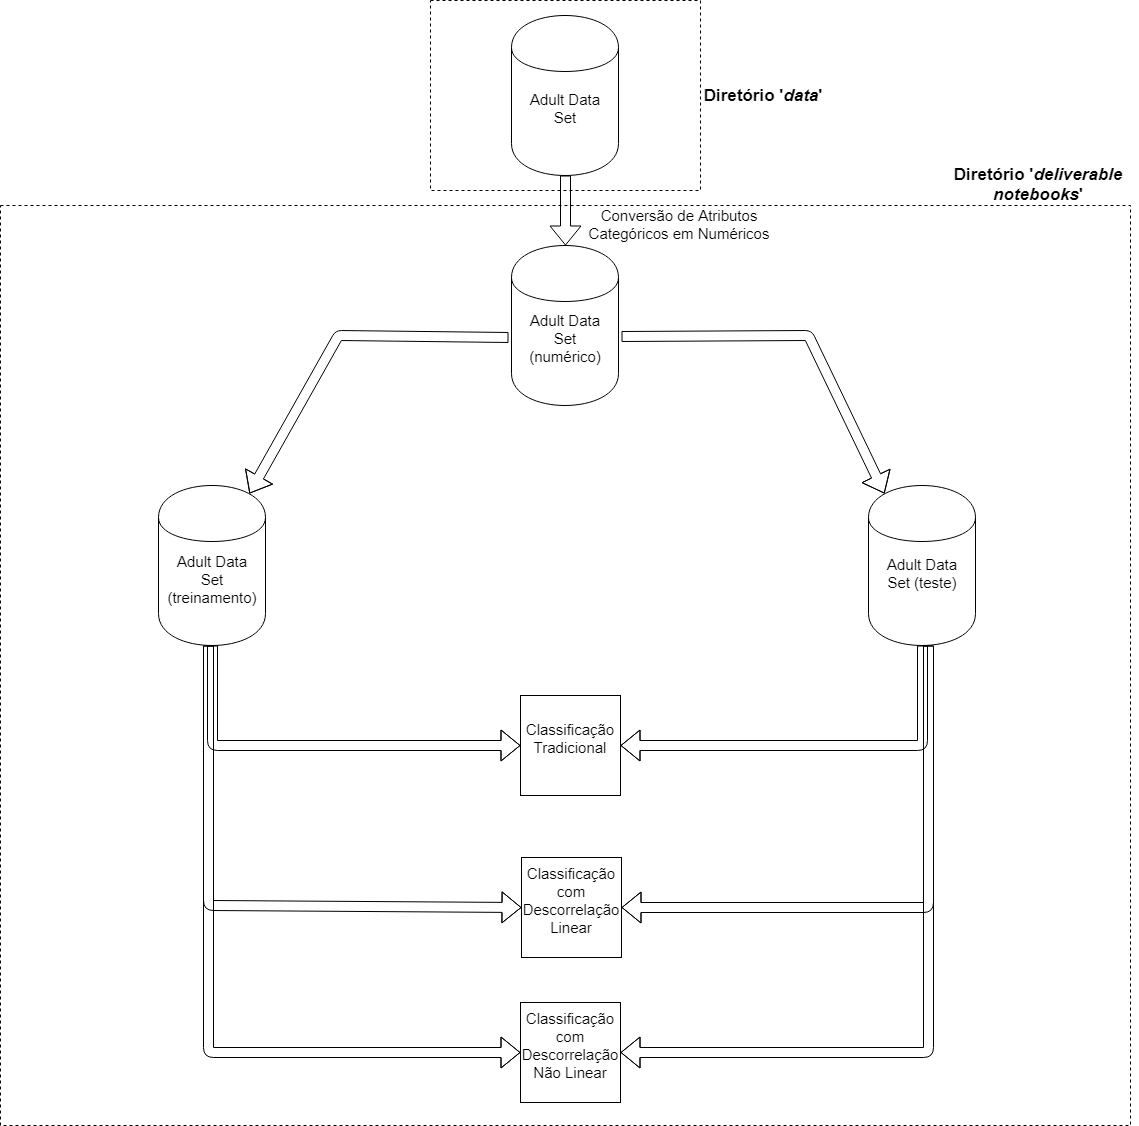
\includegraphics{../fig/WorkflowIA369.png}
\caption{Workflow}
\end{figure}

    \subsection{Resultados}\label{resultados}

Nesta seção, apresentamos nossos resultados na tarefa de classificação
em termos de acurácia e equilíbrio entre os indivíduos classificados
como "Alta Renda" nas populações masculina e feminina.

    \paragraph{Classificador 1}\label{classificador-1}

    \paragraph{Árvore de Decisão 1}\label{uxe1rvore-de-decisuxe3o-1}
\texttt{\color{outcolor}Out[{\color{outcolor}17}]:}
    
    \begin{center}
    \adjustimage{max size={0.9\linewidth}{0.9\paperheight}}{2019-05-27-dt_files/2019-05-27-dt_29_0.png}
    \end{center}
    { \hspace*{\fill} \\}
    

    \paragraph{Classificador 2}\label{classificador-2}

    \paragraph{Árvore de Decisão 2}\label{uxe1rvore-de-decisuxe3o-2}

    \paragraph{Classificador 3}\label{classificador-3}

    \paragraph{Árvore de Decisão 3}\label{uxe1rvore-de-decisuxe3o-3}

    
    \begin{verbatim}
                           Acurácia [%]
Classificador 1       76.44522932022933
Árvore de Decisão 1    82.2072072072072
Classificador 2       76.60196560196557
Árvore de Decisão 2   81.95126945126945
Classificador 3      0.7870597870597872
Árvore de Decisão 3   81.67485667485667
    \end{verbatim}

    
    Do resultado acima, notamos uma pequena perda de desempenho do
Classificador 2 para o Classificador 1, em termos de acurácia. Este tipo
de perda já é esperado, uma vez que ao reduzirmos a influência do
atributo discriminatório sobre as classes do problema, eliminamos parte
da informação de que o classificador necessita.

Esta perda de informação é muito mais acentuada no Classificador 3. Como
aplicamos a descorrelação não-linear, eliminamos de modo mais acentuado
a influência do atributo discriminatório sobre as classes do problema,
quando comparado com a redução provida pela descorrelação linear.

Na sequência, vamos avaliar como cada um dos classificadores atua na
promoção da equiadade. Para isso, avaliamos o percentual de indivíduos
classificados como "Alta Renda" em cada uma das subpopulações de
interesse.

    
    \begin{verbatim}
                     Pop. Masculina [%]   Pop. Feminina [%]
Classificador 1      34.234234234234236   6.132268632268632
Árvore de Decisão 1  21.263308763308764  3.8185913185913183
Classificador 2      16.625716625716624   3.501228501228501
Árvore de Decisão 2  20.915233415233413   4.217854217854218
Classificador 3      14.680589680589682  3.1326781326781328
Árvore de Decisão 3  20.904995904995904  4.2588042588042585
    \end{verbatim}

    
    Da tabela acima, notamos que o Classificador 2, apesar de ter uma
acurácia inferior à do Classificador 1, teve um pequeno avanço em
direção à equidade, uma vez que houve uma redução no percentual de
indivíduos da população masculina classificados como "Alta Renda" e um
acréscimo desta mesma categoria na população feminina.

Já no caso do Classificador 3, notamos um acréscimo de indivíduos
pertencentes à classe "Alta Renda" nas duas subpopulações, o que não
caminha em direção à equidade.

Para o cenário que estudamos, ambas as estratégias para mitigar o efeito
do atributo discriminatório levaram a uma queda da acurácia, como
esperado. Contudo, a decorrelação linear permitiu avanços em direção à
equidade, algo que não observamos na versão não linear (Classificador
3).

    \subsection{Conclusões}\label{conclusuxf5es}

Neste trabalho avaliamos como algumas das técnicas de ICA, \emph{i.e},
descorrelação linear e descorrelação não-linear, podem ser usadas para
promover a equidade na tarefa de classificação. Para o caso particular
que estudamos, ambas as técnicas levaram a uma redução de acurácia nos
classificadores. Contudo, a descorrelação linear levou a uma pequena
aproximação entre as populações masculina e feminina, em termos de
indivíduos classificados como "Alta Renda". Não observamos a mesma
aproximação para quando empregamos a descorrelação não-linear.


    % Add a bibliography block to the postdoc
    
    
    
    \end{document}
